\documentclass[a4paper,12pt]{article} 
\usepackage[T2A]{fontenc}			
\usepackage[utf8]{inputenc}			
\usepackage[english,russian]{babel}	
\usepackage{amsmath,amsfonts,amssymb,amsthm,mathtools} 
\usepackage[colorlinks, linkcolor = blue]{hyperref}
\usepackage{upgreek}
\usepackage[left=2cm,right=2cm,top=2cm,bottom=3cm,bindingoffset=0cm]{geometry}
\usepackage{multirow}
\usepackage{graphicx}
\usepackage{xcolor}
\usepackage{multirow}
\usepackage{pgfplots}
\usepackage{pgfplotstable}
\pgfplotsset{compat=1.9}

\pgfplotstableset{ %
        create on use/SquareLight/.style={
                create col/expr={\thisrow{Dark}}}
}

\author{Шелихов Дмитрий\\Группа Б01-305}

\title{\textbf{Работа 3.6.1\\Cпектральный анализ электрических сигналов}} 
\date{\today}

\begin{document} 

\maketitle

\textbf{Цель работы:} изучить спектры сигналов различной формы и влияние параметров сигнала на вид соответствующих спектров; проверить справедливость соотношений неопределённостей; познакомиться с работой спектральных фильтров на примере RC-цепочки. \\
\par
\textbf{В работе используются:} генератор сигналов произвольной формы, цифровой осциллограф с функцией быстрого преобразования Фурье или цифровой USB-осциллограф, подключенный к персональному компьютеру.\\
\noindent\textbf{Теоретическая справка}

По теореме Фурье любая периодическая функция может быть представлена в виде ряда (конечного или бесконечного) гармонических функций с кратными частотами - ряда Фурье. Одно из представлений ряда Фурье для функции с периодом T имеет вид
$$ f(t) = \frac{A_0}{2} + \sum_{n=1}^\infty(A_ncos(2\pi\nu_nt) + B_nsin(2\pi\nu_nt), \text{ (1)} $$
,где $\nu_n$ = n$\nu_0$, $\nu_0$ = $\frac{1}{T}$, n = 1,2,... - частоты фурье-гармоник, $A_n$ и $B_n$ - коэффициенты разложения в ряд Фурье.

Коэффициенты находятся как:

$$A_n = \frac{2}{T}\int_0^Tf(t)\cdot cos(2\pi\nu_nt)dt, B_n = \frac{2}{T}\int_0^Tf(t)\cdot sin(2\pi\nu_nt)dt. \text{ (2)}$$

На практике удобнее использовать эквивалентную форму записи ряда Фурье в "представлении амплитуд и фаз":

$$ f(t) = \frac{a_0}{2} + \sum_{n=1}^\infty a_ncos(2\pi\nu_nt+\varphi_n). \text{ (3)} $$, где $a_n = \sqrt{{A_n}^2 + {B_n}^2}$, а фаза определяется соотношением tg$\varphi_n$ = $\frac{B_n}{A_n}$

Соотношения неопределённостей.

Между сигналом как функцией времени f(t) и его спектром как функции частоты a($\nu$) имеется взаимосвязь. Если у сигнала f(t) есть какое-то характеристическое время $\Delta$t (например период повторения, длительность импульса, время нарастания и т.д.), то в спектре a($\nu$) в том или ином виде наблюдается характерный масштаб $\Delta\nu \sim \frac{1}{\Delta t}$ (расстояние между пиками, ширина спектра, ширина пиков и т.д.)

$$ \Delta\nu \cdot \Delta t \sim 1 \text{ (4) - соотношение неопределённостей} $$

Для любого сигнала с периодом T в спектре обязательно будут наблюдаться гармоники на расстоянии $\delta\nu$ = 1/T друг от друга. В данном случае соотношение является точным и от формы сигнала не зависит.

\textbf {Ход работы}

\noindent 1) По техническому описанию ознакомимся с устройством панели приборов: генератора сигналов произвольной формы и цифрового осциллографа/компьютерной программы, используемой для отображения сигналов с осциллографа. Изучим расположение основных кнопок и ручек настройки.

\noindent 2) Подключим один из выходов генератора к одному из каналов осциллографа и включим приборы в сеть.

\textbf {А. Исследование спектра периодической последовательности прямоугольных импульсов и проверка соотношений неопределённостей}

\begin{figure}
\center{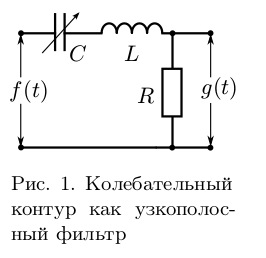
\includegraphics[width=.6\textwidth]{1.png}}
\caption{Периодическая последовательность импульсов и её спектр}
\end{figure}

\noindent 3) Следуя техническому описанию генератора, настроим генерацию прямоугольных импульсов. Параметры: $\nu_{\text{повт}}$ = 1кГц (период T = 1/$\nu_{\text{повт}}$ = 1мс), и длительность импульса $\tau$ = T/20 = 50 мкс.

\noindent 4) По техническому описанию получим устойчивую картину сигнала на экране осциллографа.

\noindent 5) Следуя техническому описанию осциллографа, получим на его экране спектр (преобразование Фурье) сигнала.

	Масштаб по горизонтальной оси установим меньше или порядка ожидаемой ширины спектра $\Delta\nu\approx$ 20 кГц  (ширину спектра оцениваем из соотношения неопределённсотей). 

	Масштаб по вертикальной оси подберём так, чтобы спектральные линии не выходили за пределы экрана (кроме, может быть, «нулевой» гармоники $\nu$ = 0 Гц, — она отвечает за уровень постоянного смещения сигнала, и ее высота может оказаться значительно выше остальных).
	
	Центр картины при предварительной настройке установите на 0 Гц, а затем после подбора масштабов сместите его так, чтобы спектр занимал весь экран начиная от левого края.

\noindent 6) Пронаблюдаем, как изменяется спектр при изменении параметров сигнала. \\

\begin{figure}
\center{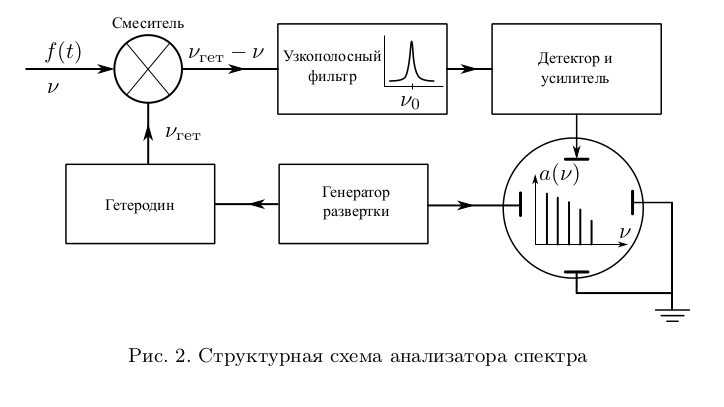
\includegraphics[width=.6\textwidth]{2.png}}
\caption{$\nu_{\text{повт}}$ = 1кГц, $\tau$ = 50мкс}
\center{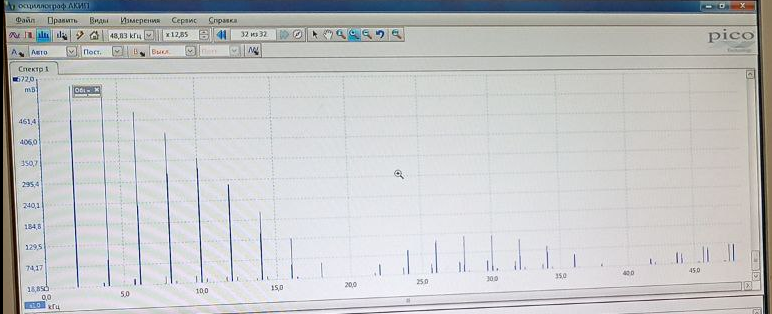
\includegraphics[width=.6\textwidth]{3.png}}
\caption{$\nu_{\text{повт}}$ = 2кГц, $\tau$ = 50мкс}
\center{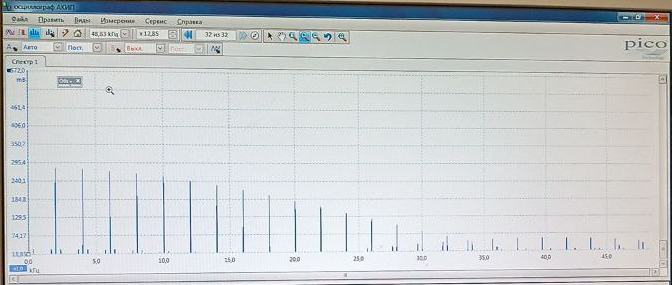
\includegraphics[width=.6\textwidth]{4.png}}
\caption{$\nu_{\text{повт}}$ = 2кГц, $\tau$ = 25мкс}
\center{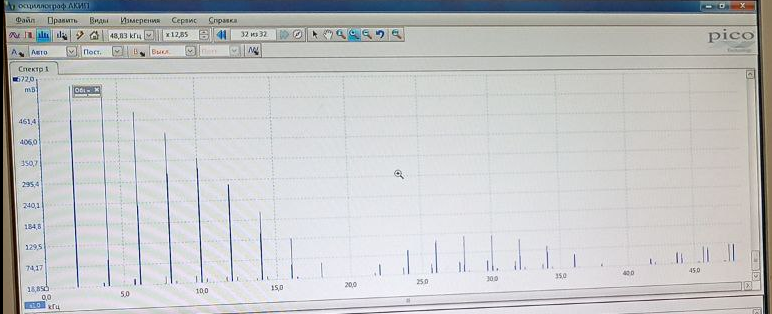
\includegraphics[width=.6\textwidth]{5.png}}
\caption{$\nu_{\text{повт}}$ = 0.5кГц, $\tau$ = 200мкс}
\end{figure}

Наблюдения: а) При увеличении $\nu_{\text{повт}}$ выросли амплитуды, ширина спектра не меняется. \\
\par        б) При увеличении $\tau$ амплитуды гармоник вырастают, а ширина спектра уменьшается. \\

\noindent 7) При фиксированных $\nu_{\text{повт}}$ = 1кГц и $\tau$ = 50мкс измерим амплитуды $a_n$ и частоты $\nu_n$ 8 гармоник. Сравним значения с рассчитанными теоретически 

$$ \nu_n = \frac{n}{T},     |a_n| = \frac{|sin\frac{\pi n\tau}{T}|}{\pi n} = \frac{\tau}{T}\frac{|sin\pi\nu_n\tau|}{\pi\nu_n\tau} $$

Результаты измерений занесём в таблицу: 

\begin{center}
\resizebox{18cm}{!}{
\begin{tabular}{|c|c|c|c|c|c|c|c|c|}
	\hline
	n гармоники & 1 & 2 & 3 & 4 & 5 & 6 & 7 & 8 \\
	\hline
	$\nu_n^{\text{эксп}}$, кГц & 1,014 & 2,031 & 3,007 & 4,024 & 5,041 & 6,017 & 6,994 & 8,011 \\
	\hline
	$\nu_n^{\text{теор}}$, кГц & 1 & 2 & 3 & 4 & 5 & 6 & 7 & 8 \\
	\hline
	$|a_n^{\text{эксп}}|$, мВ & 279,1 $\pm$ 0,1 & 275,8 $\pm$ 0,1 & 270,9 $\pm$ 0,1 & 262,7 $\pm$ 0,1 & 252,9 $\pm$ 0,1 & 241,4 $\pm$ 0,1 & 226,7 $\pm$ 0,1 & 212,0 $\pm$ 0,1 \\
	\hline
	${|a_n/a_1|}^{\text{эксп}}$ & 1 & 0,988 $\pm$ 0,001 & 0,967 $\pm$ 0,001 & 0,939 $\pm$ 0,001 & 0,904 $\pm$ 0,001 & 0,862 $\pm$ 0,001 & 0,814 $\pm$ 0,001 & 0,760 $\pm$ 0,001 \\
	\hline
	${|{a_n/a_1}|}^{\text{теор}}$ & 1 & 0,988 & 0,969 & 0,941 & 0,906 & 0,864 & 0,812 & 0,760 \\
	\hline
\end{tabular}
}
\end{center}

Получаем, что экспериментальное отношение амплитуд и рассчитанное теоретически совпадают с погрешностью не более 0.22\%.

\noindent 8) Зафиксируем период повторения T прямоугольного сигнала. T = 1мс, $\nu_{\text{повт}}$ = 1кГц. Изменяя длительность импульса $\tau$ в диапазоне от $\tau$ = T/50 до $\tau$ = T/5, измерим полную ширину спектра сигнала $\Delta\nu$ - от центра спектра ($\nu$ = 0) до гармоники с нулевой амплитудой $a_n\approx 0$.


\begin{center}
\begin{tabular}{|c|c|c|}
	\hline
	$\tau$, мкс & $\Delta\nu$, кГц & $\nu_{\text{повт}}$, кГц \\
	\hline
	30 & 27,8 $\pm$ 1.4  & \multirow{6}{*}{1}\\
	\cline{1-2} 45 & 19,9 $\pm$ 1.0 & \\
	\cline{1-2} 67,5 & 13,8 $\pm$ 0.7 & \\
	\cline{1-2} 100 & 10.0 $\pm$ 0.5 & \\
	\cline{1-2} 140 & 6,0 $\pm$ 0.3 & \\
	\cline{1-2} 200 & 5,0 $\pm$ 0.1 & \\
	\hline
\end{tabular}
\end{center}

\noindent 9) Зафиксируем длительность импульса прямоугольного сигнала $\tau$ = 100мкс. Изменяя период повторения T в диапазоне от 2$\tau$ до 50$\tau$ измерим расстояния $\delta\nu$ = $\nu_{n+1}$ - $\nu_n$ между соседнимим гармониками спектра. Если спектральные компоненты окажутся расположены слишком близко друг к другу, измерим расстояние между (n + m)-й и m-й гармониками (для некоторых целых n и m) и найдем $\delta\nu$ = $\frac{(\nu_{n+m}-\nu_n)}{m}$. 

\begin{center}
\begin{tabular}{|c|c|c|c|c|}
	\hline
	T, мкс & $\delta\nu_m$, кГц & $\delta\nu$, кГц & $\nu_{\text{повт}}$, кГц & m, шт \\
	\hline
	200 & 19,98 $\pm$ 0,02 & 4,995 $\pm$ 0,005 & 5,00 & 4 \\
	\hline
	300 & 19,98 $\pm$ 0,02 & 3,330 $\pm$ 0,003  & 3,33 & 6 \\
	\hline
	500 & 20,00 $\pm$ 0,02 & 2,000 $\pm$ 0,002 & 2,00 & 10 \\
	\hline
	800 & 12,52 $\pm$ 0,02 & 1,252 $\pm$ 0,002  & 1,25 & 10 \\
	\hline
	1100 & 9,10 $\pm$ 0,02 & 0,910 $\pm$ 0,002  & 0,91 & 10 \\
	\hline
	1500 & 6,66 $\pm$ 0,02  & 0,666 $\pm$ 0,002   & 0,67 & 10 \\
	\hline
	2000 & 5,06 $\pm$ 0,02  & 0,506 $\pm$ 0,002  & 0,50 & 10 \\
	\hline
	2500 & 4,00 $\pm$ 0,02  & 0,400 $\pm$ 0,002   & 0,40 & 10 \\
	\hline
	3000 & 3,34 $\pm$ 0,02  & 0,334 $\pm$ 0,002  & 0,33 & 10 \\
	\hline
	3500 & 2,86 $\pm$ 0,02  & 0,286 $\pm$ 0,002  & 0,29 & 10 \\
	\hline
	4000 & 2,50 $\pm$ 0,02  & 0,250 $\pm$ 0,002  & 0,25 & 10 \\
	\hline
	4500 & 2,22 $\pm$ 0,02  & 0,222 $\pm$ 0,002  & 0,22 & 10 \\
	\hline
	5000 & 2,00 $\pm$ 0,02  & 0,200 $\pm$ 0,002  & 0,20 & 10 \\
	\hline
\end{tabular}
\end{center}

\noindent 10) Построим графики зависимостей $\Delta\nu(1\ \tau)$ и $\delta\nu(1/T)$. Проведем наилучшие прямые и определим их наклон. 

\par График зависимости ширины спектра от обратного времени импульса $\Delta\nu(1/\tau)$ :

\pgfplotstableread{
x			y 		y-max 	y-min
5			5.0		0.1		0.1
7.14286		6.0		0.3		0.3
10			10.0	0.5		0.5
14.81481	13.8	0.7		0.7
22.22222	19.9	1.0		1.0
33.33333	27.8	1.4		1.4
}{\mytable}

\begin{tikzpicture}
\begin{axis} [
	title = $\Delta\nu(1/\tau)$,
	xlabel = {1/$\tau$, кГц},
	ylabel = {$\Delta\nu$, кГц},
	minor tick num = 2,
	grid = major
]

\addplot +[mark options = {scale = 0.1,}]
	plot [error bars/.cd, y dir=both, y explicit]
	table [y error plus=y-max, y error minus=y-min] {\mytable};

\addplot +[mark options = {scale = 0,}]
	table[row sep=\\,				%аппроксимация
   y={create col/linear regression={y=Y}}]
    {
   		X Y\\  
		33.33333  27.8 \\    
		22.22222  19.9\\   
		14.81481  13.8\\   
		10   10.0\\  
		7.14286   6.0\\    
		5   5.0\\     
    };
	\addlegendentry{
        k$\approx \pgfmathprintnumber{\pgfplotstableregressiona}$} 
\end{axis}
\end{tikzpicture}

Получили k $\approx$ 0.82 $\pm$ 0.05. По соотношению неопределённостей $k\approx\Delta\nu\cdot\tau\approx1$. Таким образом соотношение соблюдается, поскольку получена величина по порядку совпадающая с единицей.

\par График $\delta\nu$(1/T) :

\pgfplotstableread{
x			y 		y-max 	y-min
5.00		4.995	0.005	0.005
3.33		3.330	0.003 	0.003
2.00		2.000	0.002	0.002
1.25		1.252	0.002	0.002
0.91		0.910	0.002	0.002
0.67		0.666	0.002	0.002
0.50		0.506	0.002	0.002
0.40		0.400	0.002	0.002
0.33		0.334	0.002	0.002
0.29		0.286	0.002	0.002
0.25		0.250	0.002	0.002
0.22		0.222	0.002	0.002
0.20		0.200	0.002	0.002
}{\mytable}

\begin{tikzpicture}
\begin{axis} [
	title = $\delta\nu(1/T)$,
	xlabel = {1/T, кГц},
	ylabel = {$\delta\nu$, кГц},
	minor tick num = 2,
	grid = major
]

\addplot +[mark options = {scale = 0.5,}]
	plot [error bars/.cd, y dir=both, y explicit]
	table [y error plus=y-max, y error minus=y-min] {\mytable};

\addplot +[mark options = {scale = 0,}]
	table[row sep=\\,				%аппроксимация
   y={create col/linear regression={y=Y}}]
    {
   		X Y\\  
		5.00        4.995  \\
 3.33        3.330   \\
 2.00        2.000   \\
 1.25        1.252   \\
 0.91        0.910   \\
 0.67        0.666   \\
 0.50        0.506   \\
 0.40        0.400   \\
 0.33        0.334   \\
 0.29        0.286   \\
 0.25        0.250   \\
 0.22        0.222   \\
 0.20        0.200   \\
    };
	\addlegendentry{
        k$\approx \pgfmathprintnumber{\pgfplotstableregressiona}$} 
\end{axis}
\end{tikzpicture}

Таким образом получаем k = $\delta\nu\cdot$T = 1,000 $\pm$ 0,004 $\approx$ 1. Убеждаемся в справедливости соотношение неопределённостей. 

\textbf{Б.Наблюдение спектра периодической последовательности цугов}

\begin{figure}
\center{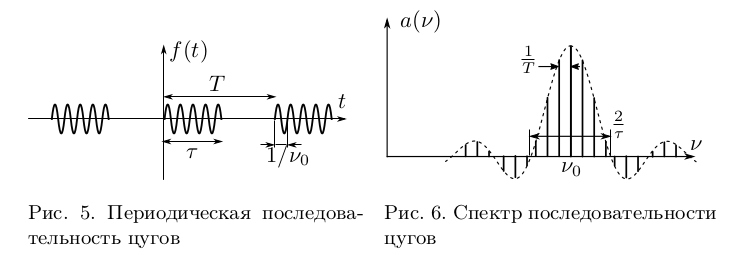
\includegraphics[width=.6\textwidth]{12.png}}
\caption{Периодическая последовательность цугов и её спектр}
\end{figure}

\noindent 11) Следуя техническому описанию генератора, установим его на режим подачи периодических импульсов синусоидальной формы ("цугов"). Установим несущую частоту $\nu_0$ = 50кГц, период повторения T = 1мс ($\nu_{\text{повт}}$ = 1кГц), число периодов синусоиды в одном импульсе N = 5 (что соответствует длительности имплульса $\tau$ = N/$\nu_0$ = 100 мкс). Получим на экране осциллографа устойчивую картину сигнала. 

\noindent 12) Получим на экране осциллографа спектр сигнала. Центр картины установим на частоту $\nu_0$. Масштаб по горизонтали (кГц/дел) подберем так, чтобы спектр помещался на экране. 

\noindent 13) Изменяя параметры сигнала T, $\nu_0$ и N пронаблюдаем, как изменяется вид спектра. Сравним наблюдаемые спектры со спектрами прямоугольных импульсов. 

\begin{figure}
\center{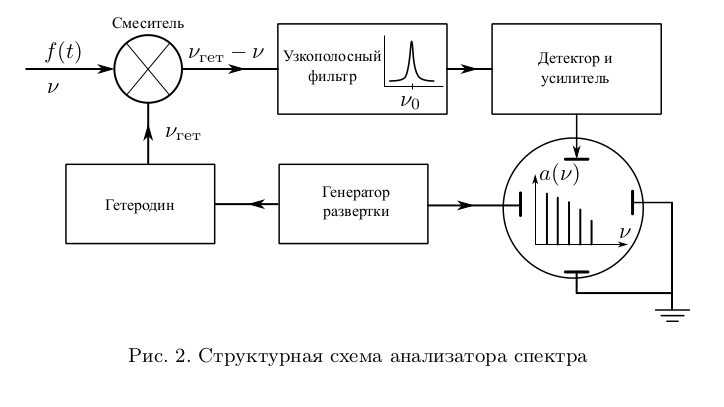
\includegraphics[width=.6\textwidth]{2.png}}
\caption{$\nu_0$ = 50кГц, T = 1мс, N = 5}
\center{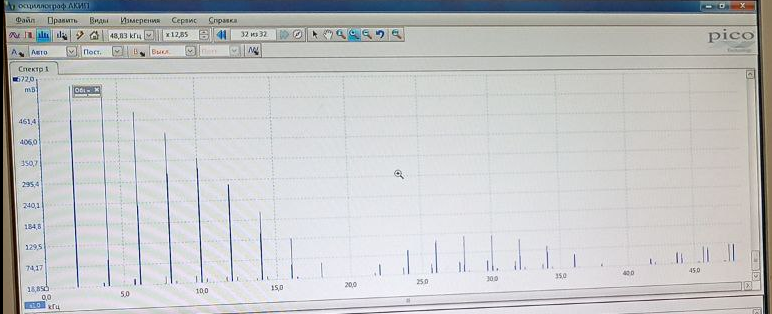
\includegraphics[width=.6\textwidth]{3.png}}
\caption{$\nu_0$ = 70кГц, T = 1мс, N = 5}
\center{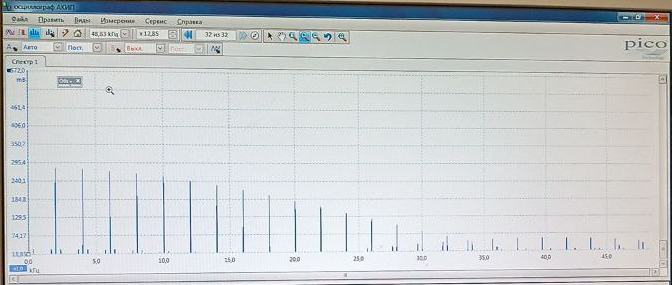
\includegraphics[width=.6\textwidth]{4.png}}
\caption{$\nu_0$ = 50кГц, T = 2мс, N = 5}
\center{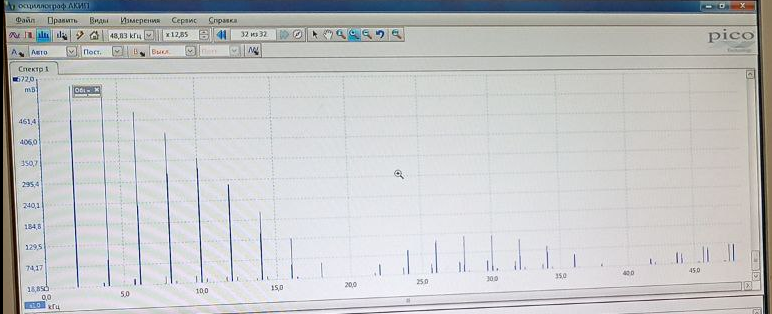
\includegraphics[width=.6\textwidth]{5.png}}
\caption{$\nu_0$ = 50кГц, T = 1мс, N = 6}
\end{figure}

Наблюдения: a) При изменении N число волн спектра равно 2N-1
\par		б) При увеличении N амплитуда растет, ширина спектра уменьшается
\par		в) При увеличении T амплитуда уменьшается, ширина спектра не меняется. Число гармоник увеличивается
\par 		г) При увеличении $\nu_0$ амплитуда уменьшается, ширина спектра растет 

\noindent 14) При параметрах сигнала, соответствующих сохранённым в предыдущем пункте изображениям, измерим положение центра спектра, его ширину $\Delta\nu$ и расстояние между гармониками $\delta\nu$.

\begin{center}
\begin{tabular}{|c|c|c|c|c|c|c|}
	\hline
	$\nu_0$, кГц & $\nu_{\text{центр}}$, кГц & T, мс & $\delta\nu_m$, кГц & m, шт & N, шт & $\delta\nu$ \\
	\hline
	50 & 50.02 $\pm$ 0.02 & 1 & 10.01 $\pm$ 0.02 & 20 & 5 & 1.00 \\
	\hline
	70 & 70.00 $\pm$ 0.02 & 1 & 14.04 $\pm$ 0.02 & 28 & 5 & 1.00  \\
	\hline
	50 & 49.94 $\pm$ 0.02 & 2 & 9.94 $\pm$ 0.02 & 40 & 5 & 0.50 \\
	\hline
	50 & 50.00 $\pm$ 0.02 & 1 & 8.00 $\pm$ 0.02 & 16 & 6 & 1.00 \\
	\hline
\end{tabular}
\end{center}

В каждом случае велчиина T$\cdot\delta\nu$ = 1. Таким образом соотношение неопределённостей выполняется. 

\textbf{Г. Исследование спектра амплитудно-модулированного сигнала}

\begin{figure}
\center{\includegraphics[width=.6\textwidth]{21.png}}
\caption{Гармонический амплитудно-модулированный сигнал и его спектр}
\end{figure}

\noindent 19) Следуя техническому описанию генератора, установим на генераторе режим модулированного по амплитуде синусоидального сигнала. Установим параметры: несущая частота $\nu_0$ = 50кГц, частота модуляции $\nu_{\text{мод}}$ = 2кГц, глубина модуляции 50\% (m = 0.5). Получим на экране осциллографа устойчивую картину сигнала. 

\noindent 20) С помощью осциллографа (в режиме курсорных измерений) измерим максимальную $A_{max}$ и минимальную $A_{min}$ амплитуды сигнала. 
Проверим справедливость равенства $m = \frac{A_{max}-A_{min}}{A_{max}+A_{min}}$

\begin{center}
\begin{tabular}{|c|c|c|c|c|c|}
	\hline
	2$A_{max}$, В & $A_{max}$, В & 2$A_{min}$, В & $A_{min}$, В  & m & $\frac{A_{max}-A_{min}}{A_{max}+A_{min}}$ \\
	\hline
	2.47 $\pm$ 0.02 & 1.24 $\pm$ 0.01 & 0.8315 $\pm$ 0.0003 & 0.4158 $\pm$ 0.0002  & 0.5 & 0.496 $\pm$ 0.008 \\
	\hline
\end{tabular}
\end{center}

В пределах погрешности экспериментально полученная глубина модуляции совпадает с выставленной. 

\noindent 21) Получим на экране спектр сигнала. С помощью осциллографа измерим частоты центральной и боковой гармоник.

\begin{center}
\begin{tabular}{|c|c|c|}
	\hline
	$\nu_{\text{бок}}$, кГц & $\nu_{\text{бок1}}$, кГц & $\nu_{\text{бок2}}$, кГц \\
	\hline
	49.99 $\pm$ 0.01 & 48 & 52 \\
	\hline
\end{tabular}
\end{center}

Изменяя несущую частоту $\nu_0$ и частоту модуляции $\nu_{\text{мод}}$ видим, что :\\
\par a) При увеличении $\nu_{\text{мод}}$ расстояние между центральной и боковой гармоникой увеличичвается. Амплитуды не меняются, центр спектра неподвижен.
\par б) При увеличении $\nu_0$ центр спектра смещается вправо, амплитуды не изменяются. 

\noindent 22) Изменяя на генераторе глубину модуляции m в диапазоне от 10\% до 100\%, измерим отношение амплитуд боковой и основной спектральных линий $a_{\text{бок}}$/$a_{\text{осн}}$. 

\begin{center}
\begin{tabular}{|c|c|c|c|}
	\hline
	 $a_{\text{осн}}$, мВ & m, \% & $a_{\text{бок}}$, мВ & $a_{\text{бок}}$/$a_{\text{осн}}$$\cdot$100, \% \\
	\hline
	 \multirow{7}{*}{582.0 $\pm$ 0.1} & 10 & 29.57 $\pm$ 0.01 & 5.08 $\pm$ 0.03 \\
	\cline{2-4}  & 20  & 59.14 $\pm$ 0.02 & 10.16 $\pm$ 0.06 \\
	\cline{2-4}  & 40  & 115.8 $\pm$ 0.04 & 19.90 $\pm$ 0.10 \\
	\cline{2-4}  & 50  & 144.1 $\pm$ 0.05 & 24.76 $\pm$ 0.12 \\
	\cline{2-4}  & 70  & 202.6 $\pm$ 0.07 & 34.81 $\pm$ 0.18 \\
	\cline{2-4}  & 80  & 229.0 $\pm$ 0.08 & 39.35 $\pm$ 0.20 \\
	\cline{2-4}  & 100  & 289.4 $\pm$ 0.10 & 49.73 $\pm$ 0.25 \\
	\hline
\end{tabular}
\end{center}

\noindent 23) Построим график $\frac{a_{\text{бок}}}{a_{\text{осн}}}$ от m и проверим, совпадает ли результат с теоретическим.

\pgfplotstableread{
x			y 		y-max 	y-min
10			5.08	0.03	0.03
20			10.16	0.06	0.06
40			19.90	0.10	0.10
50			24.76	0.12	0.12	
70			34.81	0.18	0.18
80			39.35	0.20	0.20
100			49.73 	0.25	0.25
}{\mytable}

\resizebox{\columnwidth}{!}{
\begin{tikzpicture}
\begin{axis} [
	title = $a_{\text{бок}}$/$a_{\text{осн}}$$\cdot$(m),
	xlabel = {m, \%},
	ylabel = {$a_{\text{бок}}$/$a_{\text{осн}}$$\cdot$100, \%},
	minor tick num = 2,
	grid = major
]

\addplot +[mark options = {scale = 0.1,}]
	plot [error bars/.cd, y dir=both, y explicit]
	table [y error plus=y-max, y error minus=y-min] {\mytable};

\addplot +[mark options = {scale = 0,}]
	table[row sep=\\,				%аппроксимация
   y={create col/linear regression={y=Y}}]
    {
   		X Y\\  
		10          5.08  \\
		20          10.16 \\   
		40          19.90 \\ 
		50          24.76 \\ 
		70          34.81 \\   
		80          39.35 \\  
		100			49.73 \\             
    };
	\addlegendentry{
        k$\approx \pgfmathprintnumber{\pgfplotstableregressiona}$} 
\end{axis}
\end{tikzpicture}
}

Таким образом, получаем наклон графика k$\approx$ 0.49 $\pm$ 0.01. Из теории следует, что для амплитудно-модулированного гармонического сигнала $a_{\text{бок}}$ = $\frac{m a_0}{2}$. Получили совпадение угла наклона графика в пределах погрешности.

\textbf{E.Изучение фильтрации сигналов}

\begin{figure}
\center{\includegraphics[width=.6\textwidth]{22.png}}
\caption{Схема экспериментальной установки для изучения фильтрации сигналов}
\end{figure}

\noindent 26) Для RC-цепочки с известными сопротивлением и ёмкостью рассчитаем характерное время $\tau_{RC}$ = RC и соответствующую частоту $\nu_{RC}$ = 1/$\tau_{RC}$: 

\begin{center}
\begin{tabular}{|c|c|c|c|}
	\hline
	R, кОм & C, пФ & $\tau_{RC}$, мкс & $\nu_{RC}$, кГц \\
	\hline
	3 & 1000 & 3 & 333 \\
	\hline
\end{tabular}
\end{center}

\par Соберем схему согласно рис.4. Подадим на вход RC-цепочки последовательность прямоугольных импульсов с периодом повторения T$\sim$$\tau_{RC}$ и длительностью $\tau$$\sim$T/20. 

\noindent 27) Пронаблюдаем форму сигнала и его спектр на выходе RC-цепочки("фильтрованный сигнал") при различных значениях периода T:

\begin{figure}
\center{\includegraphics[width=.6\textwidth]{14.png}}
\caption{сигнал T = 3мкс}
\end{figure}
\begin{figure}
\center{\includegraphics[width=.6\textwidth]{15.png}}
\caption{спектр T = 3мкс}
\end{figure}
\begin{figure}
\center{\includegraphics[width=.6\textwidth]{16.png}}
\caption{сигнал T = 6мкс}
\end{figure}
\begin{figure}
\center{\includegraphics[width=.6\textwidth]{17.png}}
\caption{спектр T = 6мкс}
\end{figure}
\begin{figure}
\center{\includegraphics[width=.6\textwidth]{18.png}}
\caption{сигнал T = 12мкс}
\end{figure}
\begin{figure}
\center{\includegraphics[width=.6\textwidth]{19.png}}
\caption{спектр T = 12мкс}
\end{figure}

\noindent 28) При фиксированном периоде T = 3мкс проведем измерения отношений амплитуд соответствующих спектральных гамоник фильтрованного и исходного сигналов:$K_n = |{a_n}^{\text{ф}}|/|{a_n}^{\text{0}}|$. Чтобы измерить амплитуды спектра исходного сигнала переподключим генератор к первому каналу осциллографа. 

\begin{center}
\begin{tabular}{|c|c|c|c|}
	\hline
	n & |${a_n}^{\text{0}}$|, мВ & |${a_n}^{\text{ф}}$|, мВ & $K_n$ \\
	\hline
	1 & 26.61 $\pm$ 0.02 & 8.93 $\pm$ 0.02 & 0.336 $\pm$ 0.001 \\
	\hline
	2 & 33.84 $\pm$ 0.02 & 9.23 $\pm$ 0.02 & 0.273 $\pm$ 0.001 \\
	\hline
	3 & 36.35 $\pm$ 0.02 & 9.52 $\pm$ 0.02 & 0.262 $\pm$ 0.001 \\
	\hline
	4 & 37.82 $\pm$ 0.02 & 9.23 $\pm$ 0.02 & 0.244 $\pm$ 0.001 \\
	\hline
	5 & 43.58 $\pm$ 0.02 & 9.67 $\pm$ 0.02 & 0.222 $\pm$ 0.001 \\
	\hline 
	6 & 44.17 $\pm$ 0.02 & 10.26 $\pm$ 0.02 & 0.232 $\pm$ 0.001 \\
	\hline
	7 & 45.65 $\pm$ 0.02 & 11.29 $\pm$ 0.02 & 0.247 $\pm$ 0.001 \\
	\hline
	8 & 46.24 $\pm$ 0.02 & 11.14 $\pm$ 0.02 & 0.241 $\pm$ 0.001 \\
	\hline
	9 & 49.34 $\pm$ 0.02 & 11.73 $\pm$ 0.02 & 0.238 $\pm$ 0.001 \\
	\hline
\end{tabular}
\end{center}

\noindent 29) Построим график зависимости амплитудного коэффициента фильтрации K($\nu$) от частоты $\nu$ = n$\nu_0$.

\pgfplotstableread{
x			y 		y-max 	y-min
50			0.336	0.001	0.001
100			0.273	0.001	0.001
150			0.262	0.001	0.001
200			0.244	0.001	0.001
250			0.222	0.001	0.001
300			0.232	0.001	0.001
350			0.247	0.001	0.001
400			0.241	0.001	0.001
450			0.238	0.001	0.001
}{\mytable}

\begin{tikzpicture}
\begin{axis} [
	title = $K(\nu)$,
	xlabel = {$\nu$, кГц},
	ylabel = {$K$},
	minor tick num = 2,
	grid = major
]

\addplot +[mark options = {scale = 0.1,}]
	plot [error bars/.cd, y dir=both, y explicit]
	table [y error plus=y-max, y error minus=y-min] {\mytable};

\addplot +[mark options = {scale = 0,}]
	table[row sep=\\,				%аппроксимация
   y={create col/linear regression={y=Y}}]
    {
   		X Y\\  
		 50         0.336\\
	 	100         0.273\\
	 	150         0.262\\
	 	200         0.244\\
	 	250         0.222\\
	 	300         0.232\\
	 	350         0.247\\
 	 	400         0.241\\
	 	450         0.238\\ 
    };
	\addlegendentry{
        k$\approx \pgfmathprintnumber{\pgfplotstableregressiona}$} 
\end{axis}
\end{tikzpicture}

\end{document}
